\documentclass[12pt]{article}
\usepackage{report}
\usepackage[acronym]{glossaries}
\usepackage{rotating}
\usepackage{float}
\usepackage{siunitx}
\usepackage{array}
\usepackage[justification=centering]{caption}
\usepackage{booktabs}
\usepackage[table,xcdraw]{xcolor}
\usepackage{chngcntr}
\usepackage[utf8]{inputenc}
\usepackage{listings}  % Package for code formatting
\usepackage{xcolor}    % Enables color for syntax highlighting

\lstdefinelanguage{PHP}{
    morekeywords={echo, if, else, while, for, foreach, function, return, class, public, private, protected, extends, implements, new, var, static, global},
    sensitive=true,
    morecomment=[l]{//},
    morecomment=[s]{/*}{*/},
    morestring=[b]",
    morestring=[b]'
}

\lstset{
    language=PHP, % Set the language to PHP
    basicstyle=\ttfamily\small, % Monospaced font
    keywordstyle=\color{blue}, % Keywords in blue
    commentstyle=\color{gray}, % Comments in gray
    stringstyle=\color{red}, % Strings in red
    backgroundcolor=\color{lightgray!10}, % Light gray background
    frame=single, % Add a border around the code
    breaklines=true, % Allow line breaking
    numbers=left, % Show line numbers
    numberstyle=\tiny\color{gray} % Line number styling
}

\title{Project proposal format For B.Sc. CSIT/BIT, TU, IOST}
\author{Prakash Neupane}
\date{\today}

\begin{document}
\pagenumbering{roman} % Roman page numbers

\addcontentsline{toc}{section}{TITLE PAGE}
\thispagestyle{empty} % This will hide the page number on the title page
\begin{titlepage}
    \centering
    \begin{center}
        
\includegraphics[width=0.3\textwidth]{./Images/PUClogo.png} % Adjust width as necessary
    \end{center}
\begin{center}
    \textbf{Department of Computer Science and Engineering}\\
    Premier University
\end{center}
\begin{center}
    \textnormal{ CSE 338: Software Development }
\end{center}
    \vspace{0.5in}
    \small
    \textbf{A Project Proposal Report On}\\
    \vspace{0.5in}
    \large
    \uppercase{\textbf{Odyssey Travel Agency Software}}\\
    \vspace{0.5in}
    \large
    \textbf {Submitted by}\\
    \begin{center}
        \renewcommand{\arraystretch}{1.5} % Adjusts vertical spacing in the table
        \begin{tabular}{|>{\raggedright\arraybackslash}p{0.6\textwidth}|p{0.3\textwidth}|} % Adjust column widths
        \hline
        \textbf{Name} & \textbf{ID} \\
        \hline
        Mohammad Hafizur Rahman Sakib & 0222210005101118 \\
        \hline
        Arnab Shikder & 0222210005101098 \\
        \hline
        Sayed Hossain & 0222210005101102 \\
        \hline
        Mohammad Asmual Hoque Yousha & 0222210005101121 \\
        \hline
        \end{tabular}
        \end{center}
    \vspace{0.5in}
 
\begin{minipage}[t]{0.5\textwidth}
        \textbf{Submitted to :}
        \\Tashin Hossain
        \\Lecturer,Department of CSE
        \\ Premier University
        \\ Chittagong
    \end{minipage}%
    \begin{minipage}[t]{0.6\textwidth}
        \raggedleft
        \textbf{Remarks}\\
        \vspace{0.5cm} % Adjust vertical space for remarks
        \begin{tikzpicture}
            \draw[thick, rounded corners] (0,0) rectangle (4,2);
        \end{tikzpicture}
    \end{minipage}

    \date{\today}
    \vfill
\end{titlepage}


\newpage % Ensure this file exists and is correctly formatted

% Table of contents
\newpage
{
  \setlength{\parskip}{0em}
  \renewcommand\contentsname{TABLE OF CONTENTS} % This will change heading text
  \tableofcontents \addcontentsline{toc}{section}{TABLE OF CONTENTS}
}

% List of figures - if any
\newpage
\listoffigures 
\addcontentsline{toc}{section}{LIST OF FIGURES}

% List of tables - if any
\newpage
\listoftables 
\addcontentsline{toc}{section}{LIST OF TABLES}
\pagenumbering{arabic}

\clearpage
\thispagestyle{plain}
\begin{center}
    \LARGE{\textbf{Abstract}}
\end{center}
The “Odyssey Travel Agency Software” is a full-stack web application designed to simplify and enhance the travel booking process for users and administrators alike. Users can register, browse country-specific tour packages, select desired packages, choose flight and hotel preferences, and proceed to book through a secure payment gateway. The frontend leverages HTML, CSS, Tailwind CSS, JavaScript, and Next.js for a responsive and interactive user experience, while the backend is powered by Laravel and MySQL for efficient data processing and management. The admin interface allows CRUD operations on tour packages and facilitates the addition of local tour guide details. The system is developed following core software engineering principles such as modularity, scalability, and user-centric design, ensuring the product is both robust and maintainable for long-term use.

\textbf{Keywords:} Travel Booking System, Laravel, Next.js, Tour Packages, Full-Stack Web Application, Payment Gateway, Admin Panel, CRUD Operations

\vspace{0.5cm}

\noindent GitHub Repository:
\href{https://github.com/ArnabShikder24/odyssey-travel-client}{\textbf{https://github.com/ArnabShikder24/odyssey-travel-client}} 



\section{Background}
Cassava is a staple food crop grown in tropical and subtropical regions. It is valued for its high-yield tubers and nutrient-rich leaves. Its resilience in poor soils makes it a vital food source in many low-income regions. However, cassava plants are highly susceptible to several leaf diseases including Cassava Bacterial Blight (CBB), Cassava Brown Streak Disease (CBSD), Cassava Green Mottle (CGM), and Cassava Mosaic Disease (CMD). These diseases disrupt the photosynthetic process and significantly reduce crop yield and quality.

Conventional methods of disease detection involve laboratory testing or expert consultation, both of which are costly and time-consuming. As a result, farmers often lack the means to detect and treat diseases early. With recent advances in machine learning, especially in image classification using deep learning, it is now possible to build systems that can classify crop diseases from images with high accuracy and low cost. This project applies such techniques to develop a cassava leaf disease detection system.

\section{Problem Statement}
In regions like Bangladesh, where cassava is not yet widely cultivated but has strong potential, there is limited infrastructure for disease monitoring. Farmers lack tools for early and accurate identification of leaf diseases. Manual diagnosis is often not viable due to lack of expertise, cost, and time constraints.

This research focuses on the classification of cassava leaf diseases using machine learning models trained on labeled image datasets. The goal is to evaluate various deep learning models to determine which provides the best trade-off between accuracy and computational efficiency, ultimately aiding in timely and scalable disease detection.

\section{Chapter Distribution}
This report is organized into the following chapters:

\begin{itemize}
    \item \textbf{Chapter 1: Introduction} — Introduces the background of the study, identifies the research problem, and outlines the structure of the report.
    
    \item \textbf{Chapter 2: Literature Review} — Summarizes related works from at least eight research papers relevant to crop disease classification, focusing on methods, datasets, and performance metrics.

    \item \textbf{Chapter 3: Methodology} — Describes the overall method used in the project, details the machine learning models implemented, and explains the proposed framework that yielded the best performance.

    \item \textbf{Chapter 4: Experimental Result and Analysis} — Provides a description of the dataset, evaluation metrics, and parameter settings. It also discusses experimental results in detail, including error analysis, limitations, and the social or cultural impact of the proposed solution.

    \item \textbf{Chapter 5: Conclusion and Future Work} — Summarizes the research findings, reflects on the limitations, and suggests directions for future improvements and further study.
\end{itemize}

 % Ensure this file exists and is correctly formatted
\section{Literature Review}

\section{Methodology}
This section outlines the systematic approach followed during the development of the travel agency website. The Software Development Life Cycle (SDLC) model was followed to ensure that the project was well-organized, efficient, and delivered successfully within the given timeframe.

\subsection{Planning}
The planning phase involved identifying project goals, features, and tools. The stack was finalized to include HTML, Tailwind CSS, JavaScript, and Next.js for the frontend, and Laravel with MySQL for the backend. Requirements were gathered for both the user and admin roles, and the expected user journey was mapped out—from viewing packages to payment completion.

\subsection{Design}
The design phase included both frontend and backend architectural planning. Wireframes were drawn to visualize page layouts such as Home, Package Listing, and Booking pages. The backend was structured using Laravel's MVC architecture. ER diagrams were created to model database relationships for users, packages, bookings, and tour guides.

\subsection{Implementation}
Frontend pages were built using Next.js for server-side rendering and faster load times. Tailwind CSS was used for consistent, responsive styling. On the backend, Laravel handled routing, controllers, models, and database migrations. Admin features like CRUD operations for tour packages and guide management were also implemented here.

\subsection{Testing}
Unit and integration testing were carried out to ensure all features worked as intended. Laravel’s built-in testing tools were used to test backend logic. Frontend behavior was manually tested across different browsers and devices. Form validation and session handling were thoroughly checked.

\subsection{Deployment}
After successful testing, the application was prepared for deployment. The backend (Laravel) was hosted on a PHP-compatible server, and the Next.js frontend was deployed via Vercel or a Node-compatible server. Environment variables were configured for secure communication with the database and third-party services.

\subsection{Future Enhancements}
Possible future improvements include integrating a real-time chatbot for customer support, adding review and rating features for packages, incorporating real-time availability for flights and hotels via APIs, and building a mobile app version of the platform using React Native.

%\newpage
\section{Diagrams}

\subsection{UML (Unified Modeling Language)}
UML (Unified Modeling Language) is a standardized modeling language used to visualize, design, and document the structure and behavior of software systems. It provides a graphical representation of the system architecture, relationships, and interactions between components.

\vspace{0.5cm}
\begin{center}
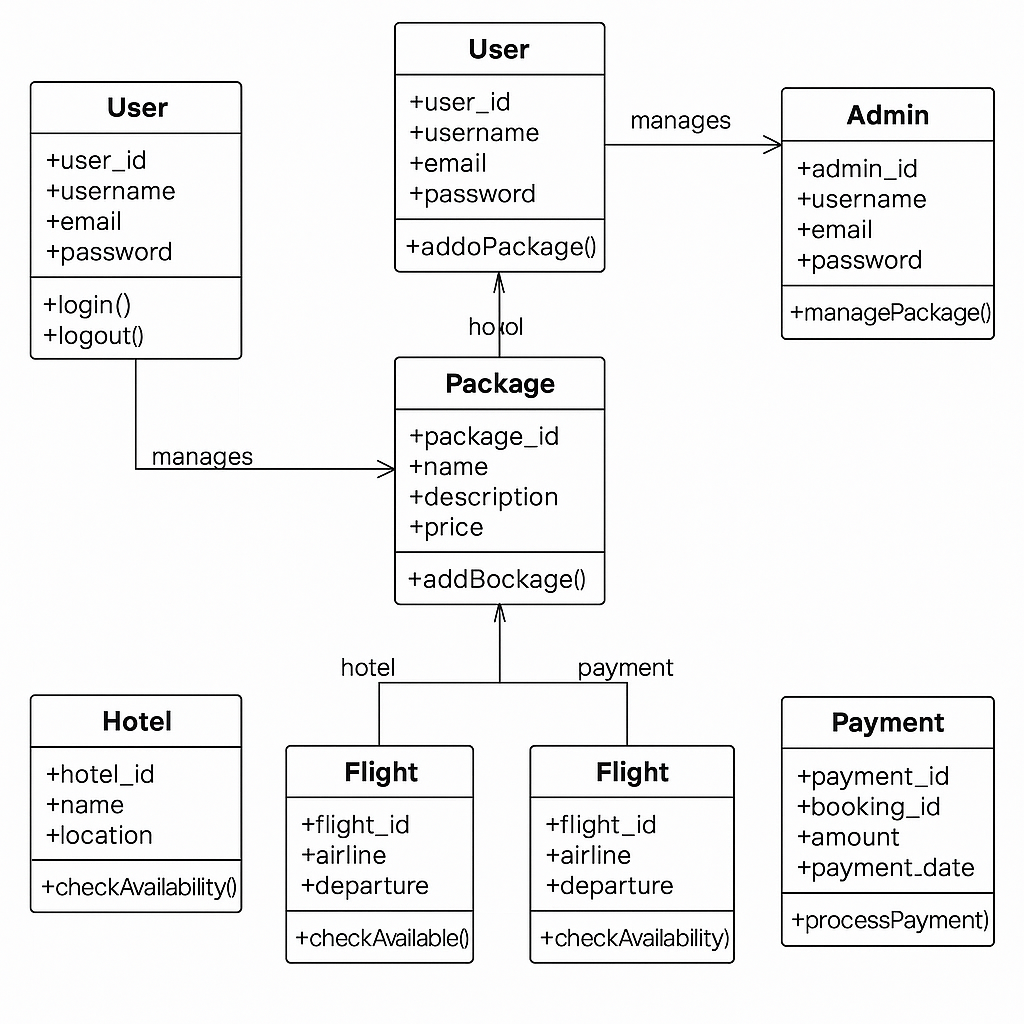
\includegraphics[width=1.0\textwidth]{./figures/UML Diagram/uml2.0.png} % Replace with your actual UML diagram path
\captionof{figure}{UML Diagram}
\end{center}
\vspace{0.5cm}

\subsection{Activity Diagram}
\subsubsection{Description}
An Activity Diagram models the flow of control in a system, representing the sequence of activities and their transitions. It visually represents workflows such as business processes or the flow of an algorithm, using actions, decisions, start and end points, and parallel processing.

\subsubsection{Usage}
\begin{itemize}
    \item \textbf{Workflow Representation:} Used to model high-level business processes or system workflows.
    \item \textbf{Decision Making:} Helps in visualizing conditional logic, showing decision points and alternative flows.
    \item \textbf{Parallel Processes:} Represents parallel processing or branching in a system.
\end{itemize}

\subsubsection{Key Elements}
\begin{itemize}
    \item \textbf{Initial Node:} Marks the starting point of the process.
    \item \textbf{Activity/Action:} Represents tasks or operations performed.
    \item \textbf{Decision Node:} Represents branching in the workflow, where a choice must be made.
    \item \textbf{Merge Node:} Combines multiple flows back into a single flow after decision points.
    \item \textbf{Final Node:} Marks the end of the process.
\end{itemize}

\vspace{0.5cm}
\begin{center}
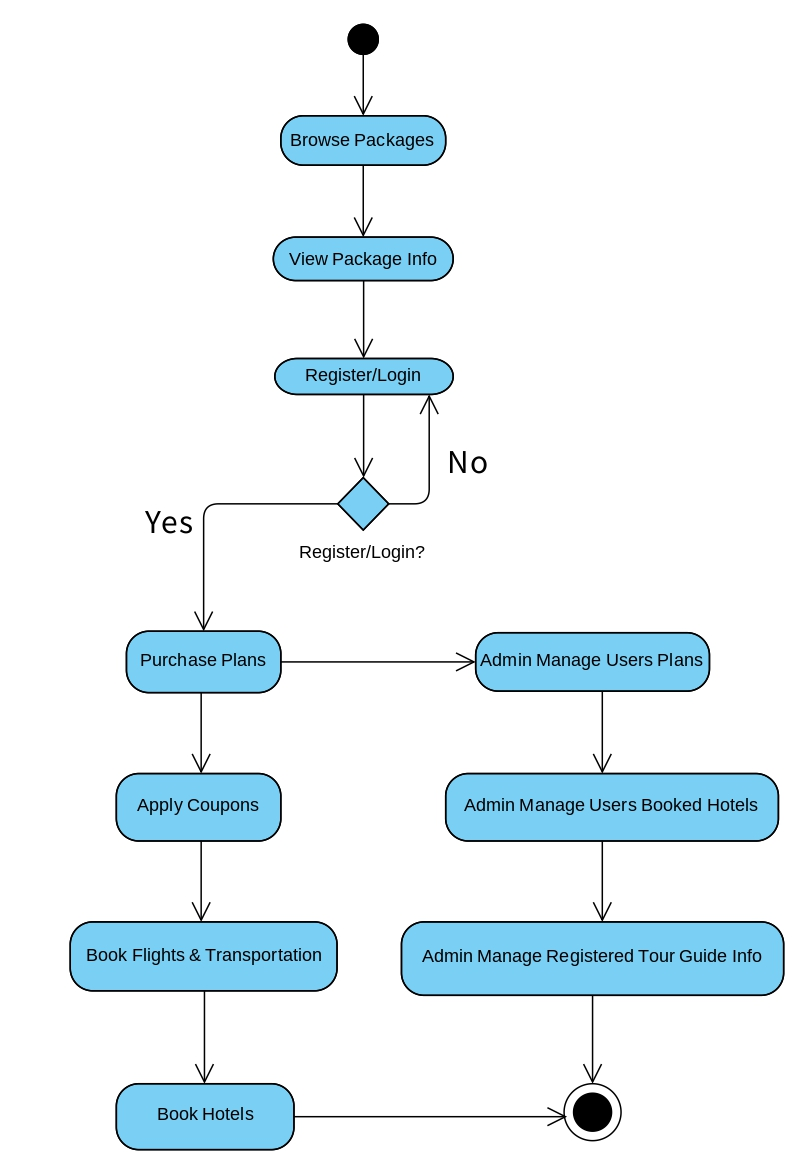
\includegraphics[width=1.0\textwidth]{./figures/Activity Diagram/actd.jpg} % Replace with your actual Activity Diagram path
\captionof{figure}{Activity Diagram for Odyssey Travel Agency Software}
\end{center}
\vspace{0.5cm}


\vspace{0.5cm}
\begin{center}
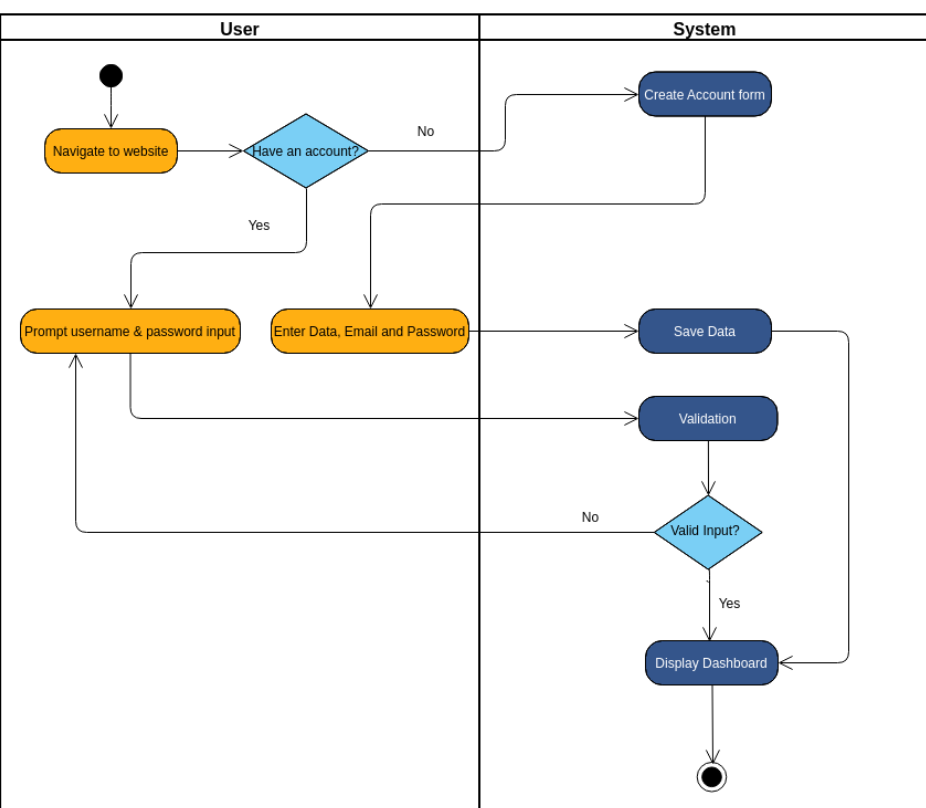
\includegraphics[width=0.8\textwidth]{./figures/Activity Diagram/1_reg.png} % Replace with your actual Activity Diagram path
\captionof{figure}{Activity Diagram Of Login and Registra   tion System} 
\end{center}
\vspace{0.5cm}

\vspace{0.5cm}
\begin{center}
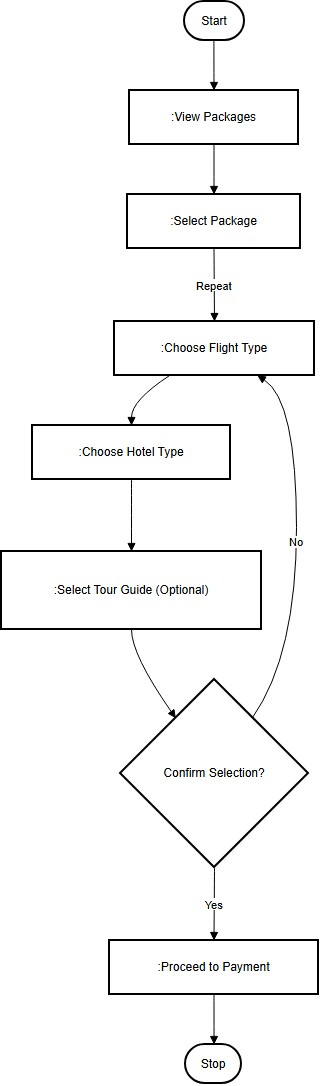
\includegraphics[width=0.5\textwidth]{./figures/Activity Diagram/2_activity.jpg} % Replace with your actual Activity Diagram path
\captionof{figure}{Package Selection Activity Diagram}
\end{center}
\vspace{0.5cm}

\vspace{0.5cm}
\begin{center}
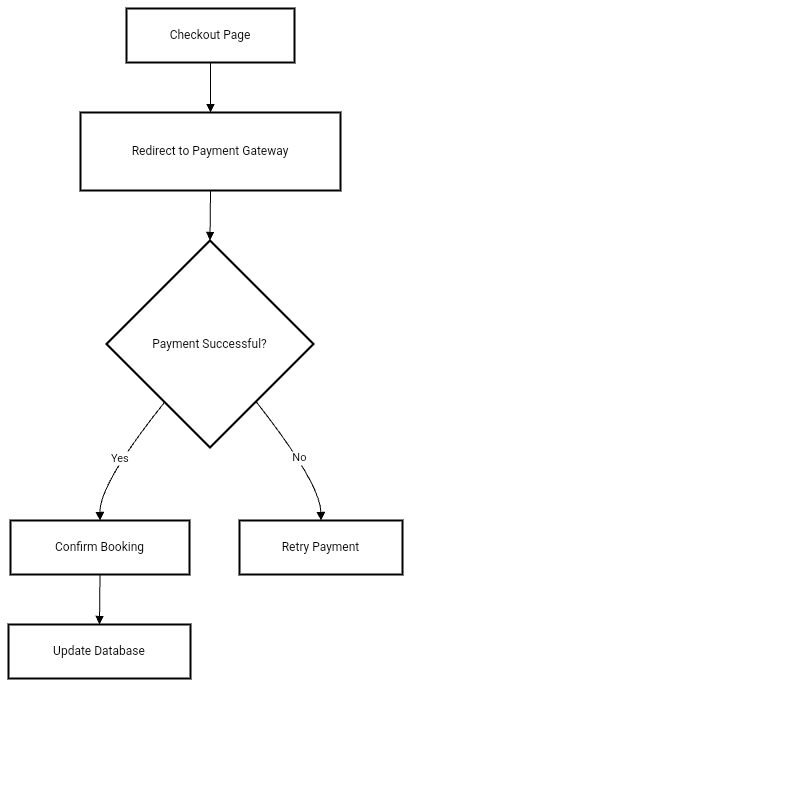
\includegraphics[width=0.8\textwidth]{./figures/Activity Diagram/3_acivity.png} % Replace with your actual Activity Diagram path
\captionof{figure}{Payment System Activity Diagram}
\end{center}
\vspace{0.5cm}

\vspace{0.5cm}
\begin{center}
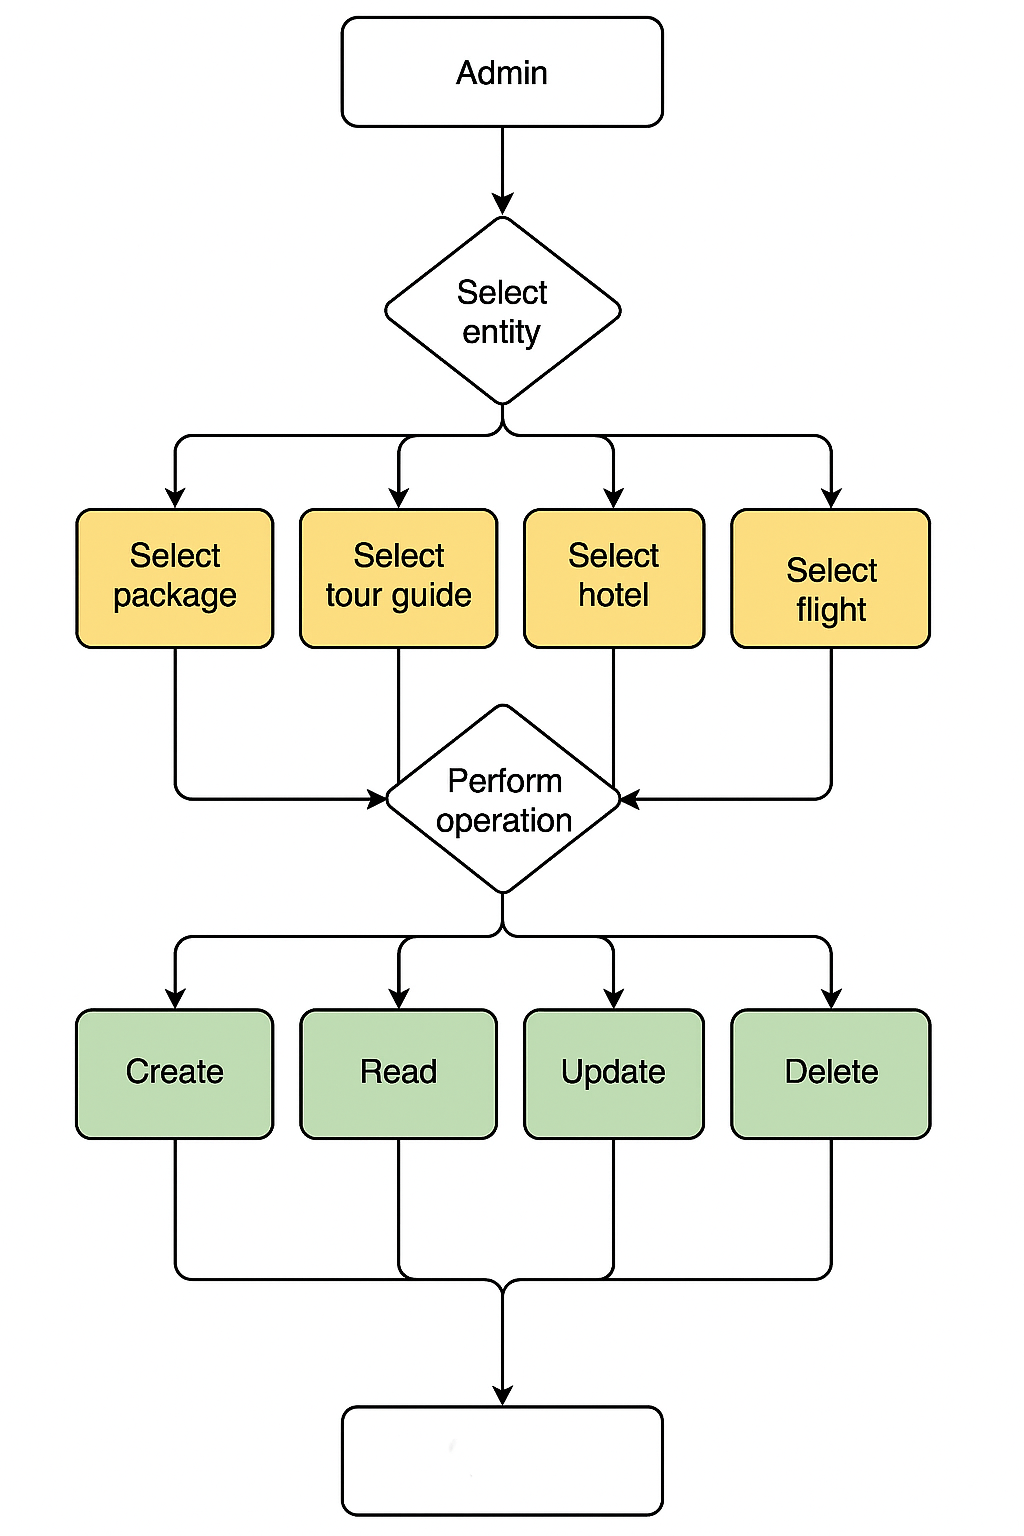
\includegraphics[width=0.8\textwidth]{./figures/Activity Diagram/4_crud_activity.png} % Replace with your actual Activity Diagram path
\captionof{figure}{Admin CRUD Operation Activity Diagram}
\end{center}
\vspace{0.5cm}


\subsection{Sequence Diagram}
\subsubsection{Description}
A Sequence Diagram focuses on the interaction between objects or components in a system over time. It shows the sequence of messages exchanged between objects to achieve a specific goal or functionality. It highlights the order of interactions and the roles of different components in a system.

\subsubsection{Usage}
\begin{itemize}
    \item \textbf{Object Interaction:} Helps in understanding the detailed interactions between different objects in a system.
    \item \textbf{Method Call Flow:} Useful for describing the flow of control during method calls and responses.
    \item \textbf{Debugging \& Testing:} Provides insight into the communication between objects, useful for debugging and designing test cases.
\end{itemize}

\subsubsection{Key Elements}
\begin{itemize}
    \item \textbf{Objects/Actors:} Represent entities that participate in the interaction.
    \item \textbf{Lifeline:} A dashed line that represents the lifespan of an object during the interaction.
    \item \textbf{Message Arrows:} Represent the messages sent between objects, showing the direction and order.
    \item \textbf{Activation Bar:} Indicates when an object is active (processing).
    \item \textbf{Return Message:} Represents the return of control from a method.
\end{itemize}

\vspace{0.5cm}
\begin{center}
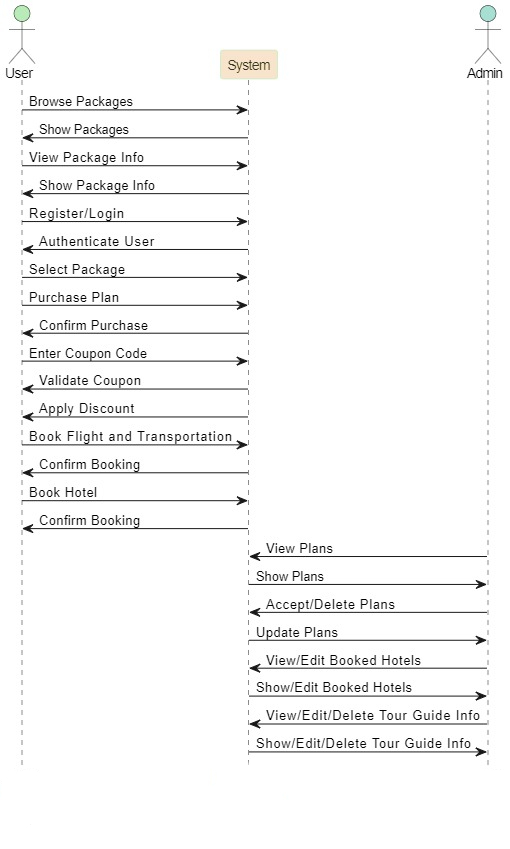
\includegraphics[width=0.8\textwidth]{./figures/Sequence Diagram/sqd.jpg} % Replace with your actual Sequence Diagram path
\captionof{figure}{Sequence Diagram of Odyssey Travel Agency Software}
\end{center}
\vspace{0.5cm}

\vspace{0.5cm}
\begin{center}
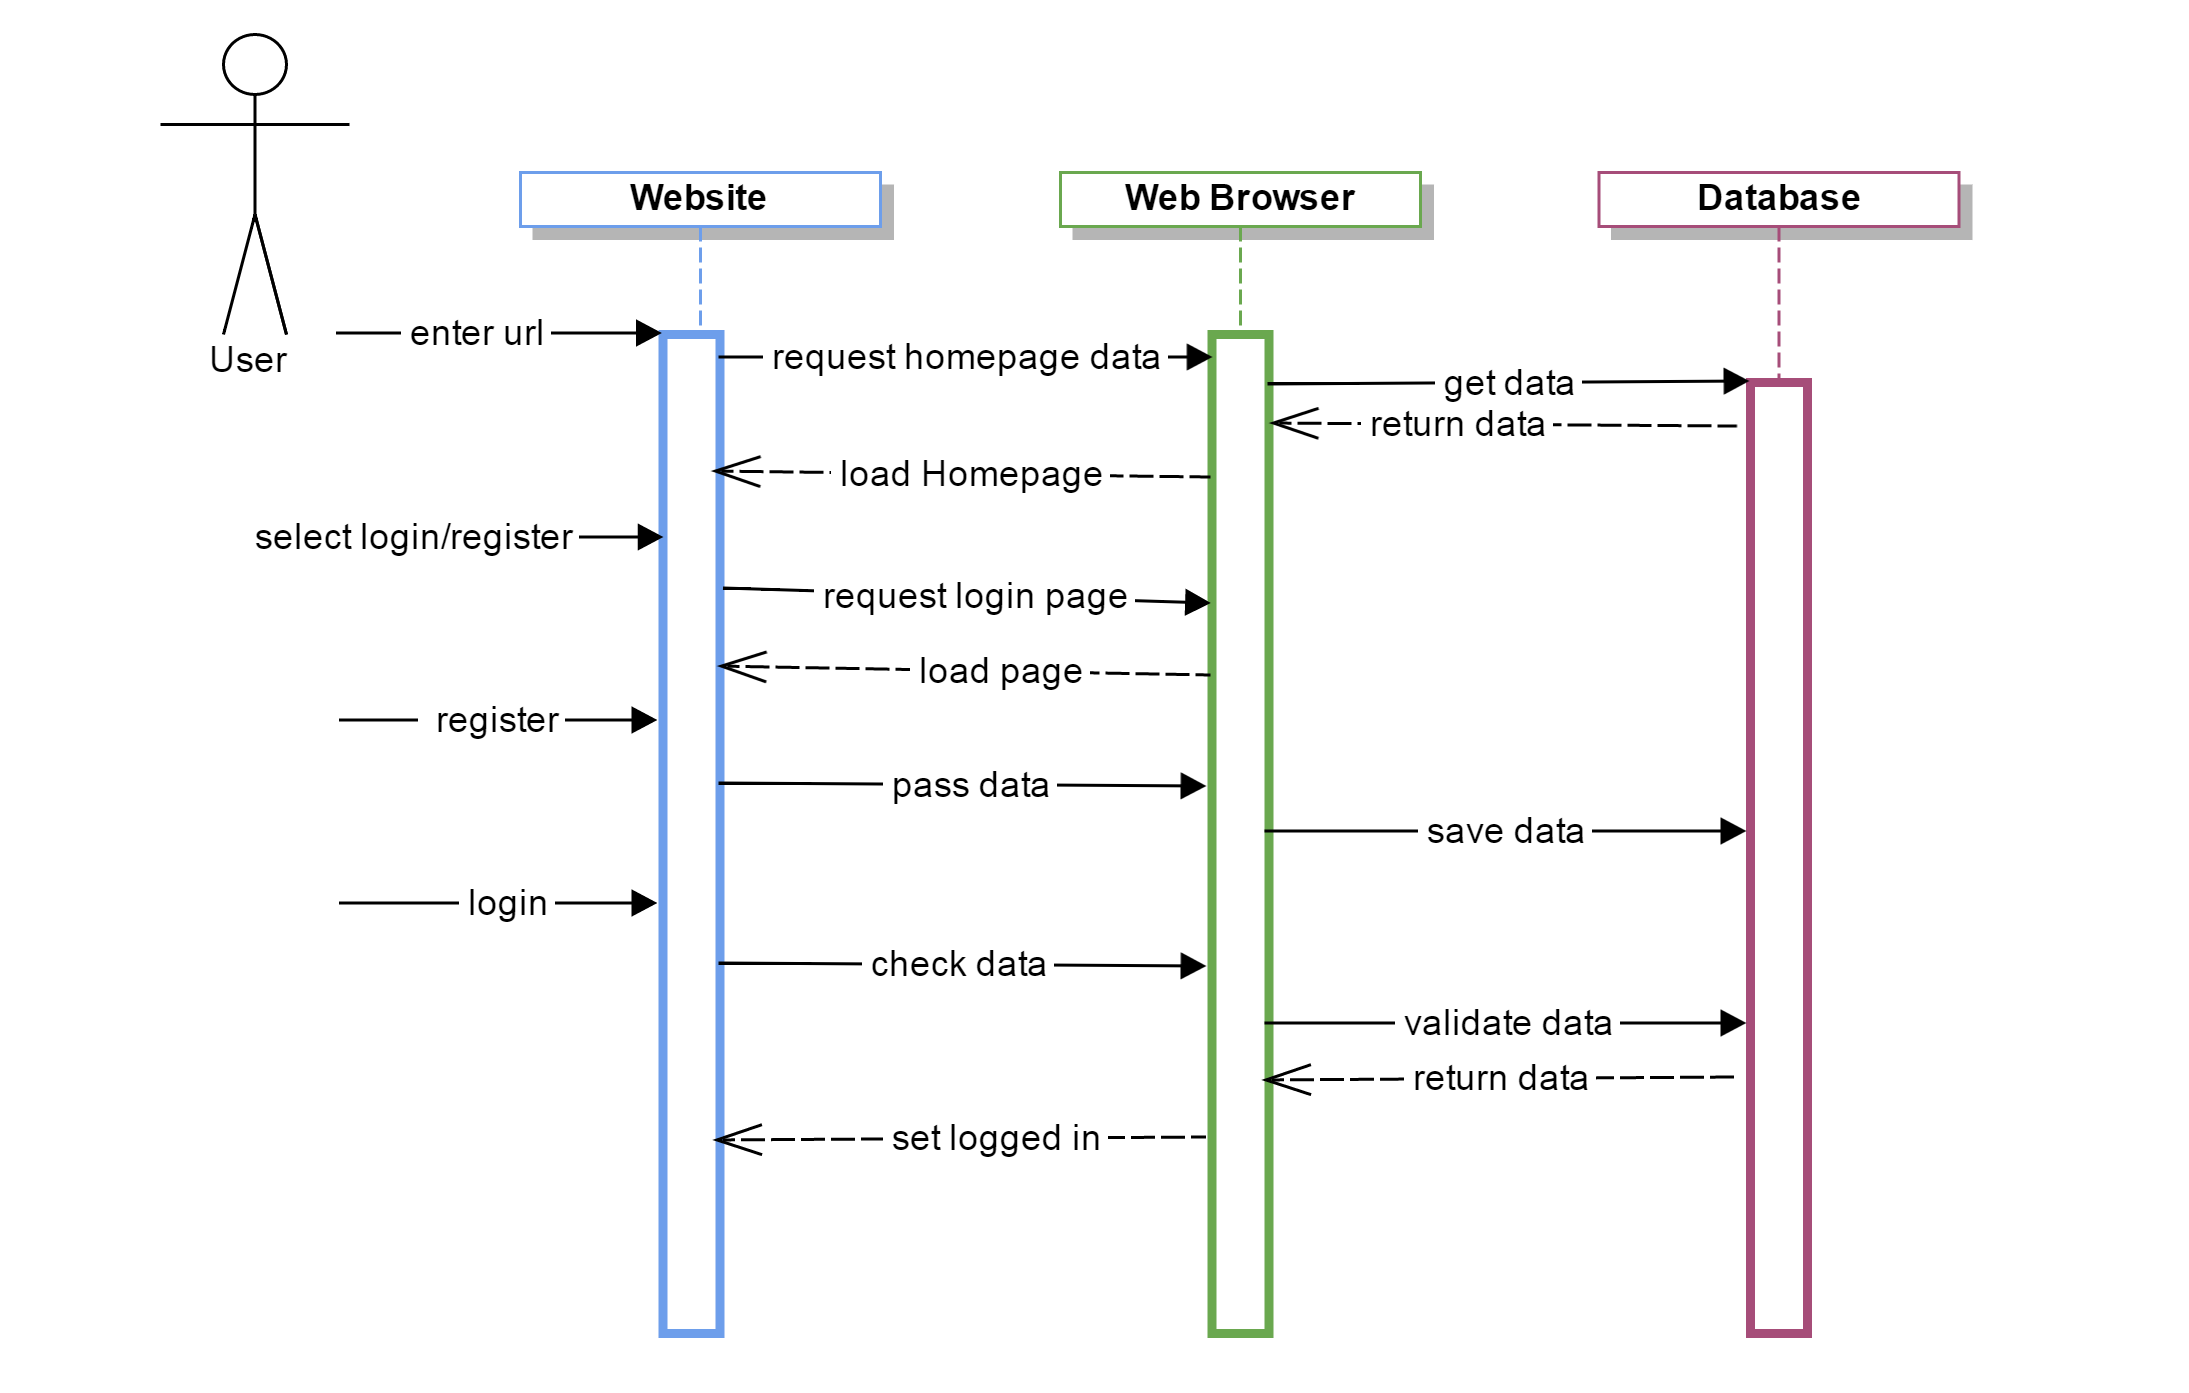
\includegraphics[width=0.9\textwidth]{./figures/Sequence Diagram/1_seq.png} % Replace with your actual Activity Diagram path
\captionof{figure}{Sequence Diagram Of Login and Registra   tion System} 
\end{center}
\vspace{0.5cm}

\vspace{0.5cm}
\begin{center}
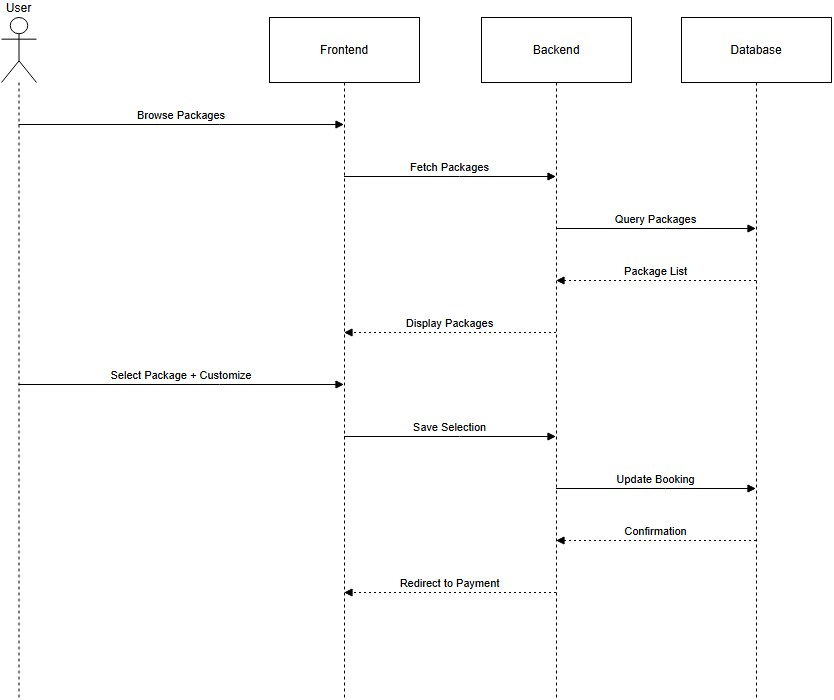
\includegraphics[width=1.0\textwidth]{./figures/Sequence Diagram/2_seq.jpg} % Replace with your actual Activity Diagram path
\captionof{figure}{Package Selection Sequence Diagram}
\end{center}
\vspace{0.5cm}

\vspace{0.5cm}
\begin{center}
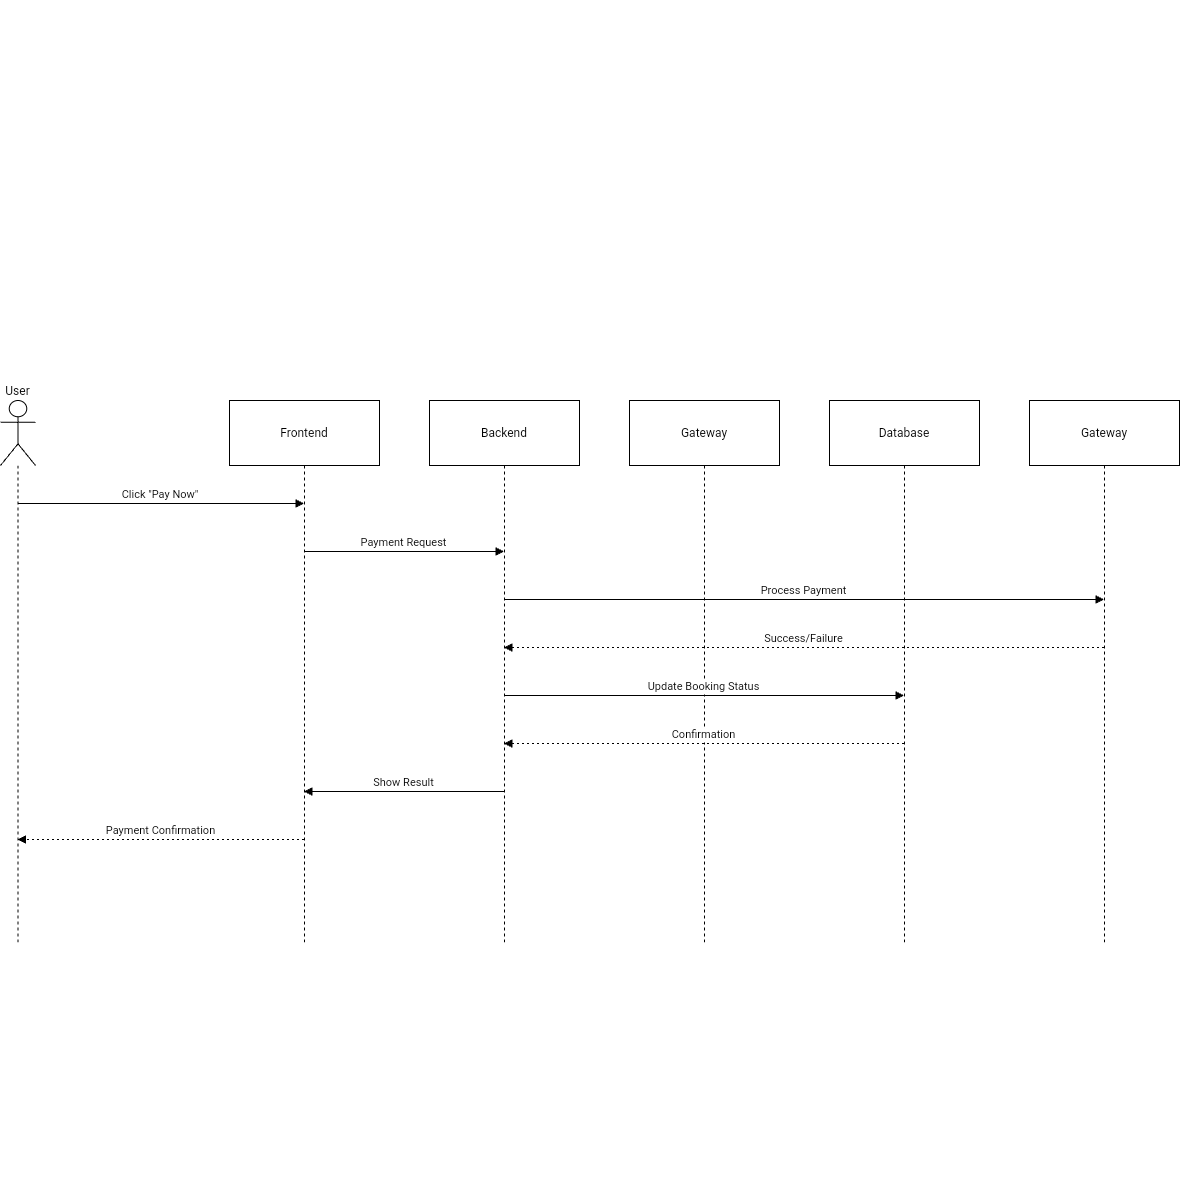
\includegraphics[width=1.0\textwidth]{./figures/Sequence Diagram/3_seq.png} % Replace with your actual Activity Diagram path
\captionof{figure}{Payment System Sequence Diagram}
\end{center}
\vspace{0.5cm}

\vspace{0.5cm}
\begin{center}
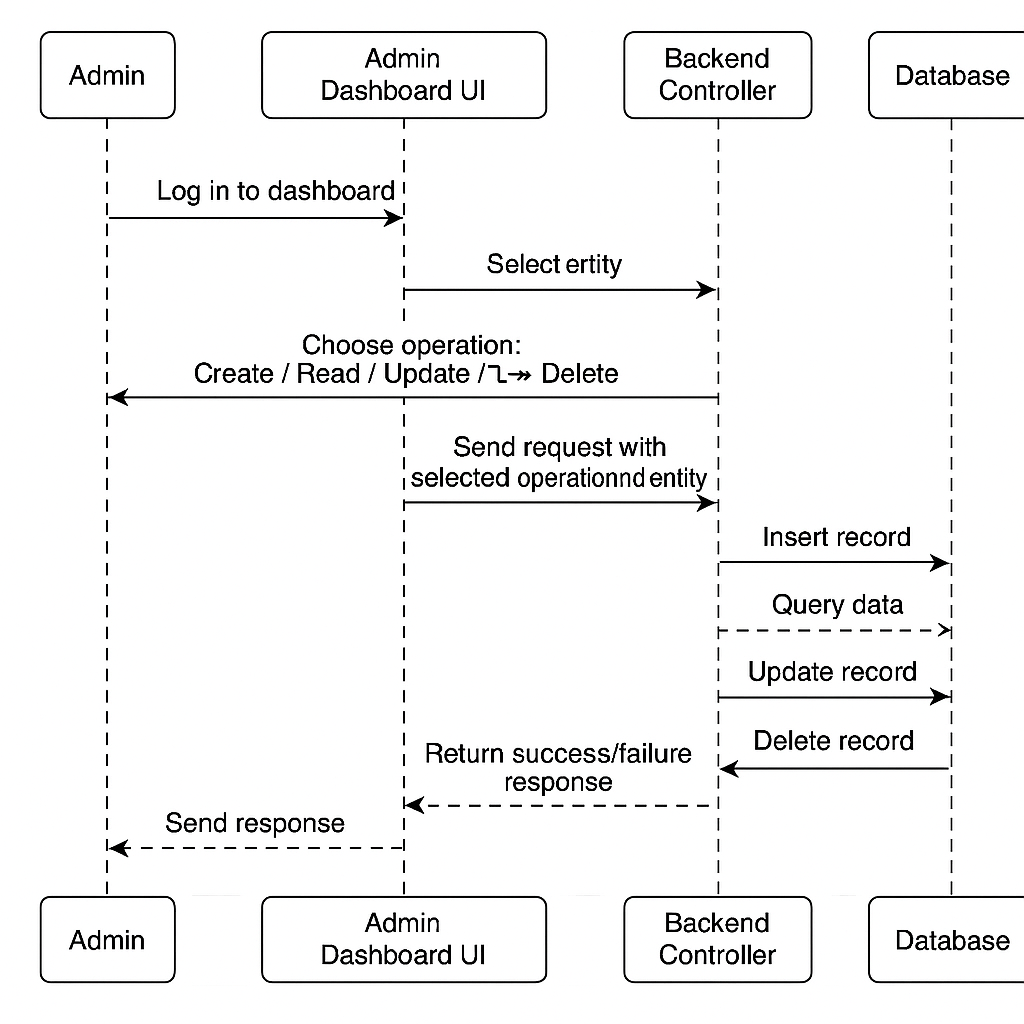
\includegraphics[width=0.8\textwidth]{./figures/Sequence Diagram/4_crud_sequence.png} % Replace with your actual Activity Diagram path
\captionof{figure}{Admin CRUD Operation Sequence Diagram}
\end{center}
\vspace{0.5cm}

\subsection{Use Case Diagram}
\subsubsection{Description}
A Use Case Diagram represents the functional requirements of a system by showing interactions between users (actors) and the system itself. It highlights the different use cases (functions or processes) the system performs and which actors are involved in each use case.

\subsubsection{Usage}
\begin{itemize}
    \item \textbf{Requirement Gathering:} Used to capture and clarify system functionality from the user's perspective.
    \item \textbf{System Scope:} Defines the boundaries of the system and what will be included in its functionality.
    \item \textbf{User Interaction:} Visualizes user-system interactions to understand how different users (actors) use the system.
\end{itemize}

\subsubsection{Key Elements}
\begin{itemize}
    \item \textbf{Actors:} Represent users or other systems that interact with the system.
    \item \textbf{Use Cases:} Represent functions or actions that the system performs (e.g., "Login," "Add Package").
    \item \textbf{System Boundary:} Represents the scope of the system and distinguishes between internal functions and external actors.
    \item \textbf{Associations:} Arrows or lines connecting actors to use cases, indicating their involvement.
\end{itemize}

\vspace{0.5cm}
\begin{center}
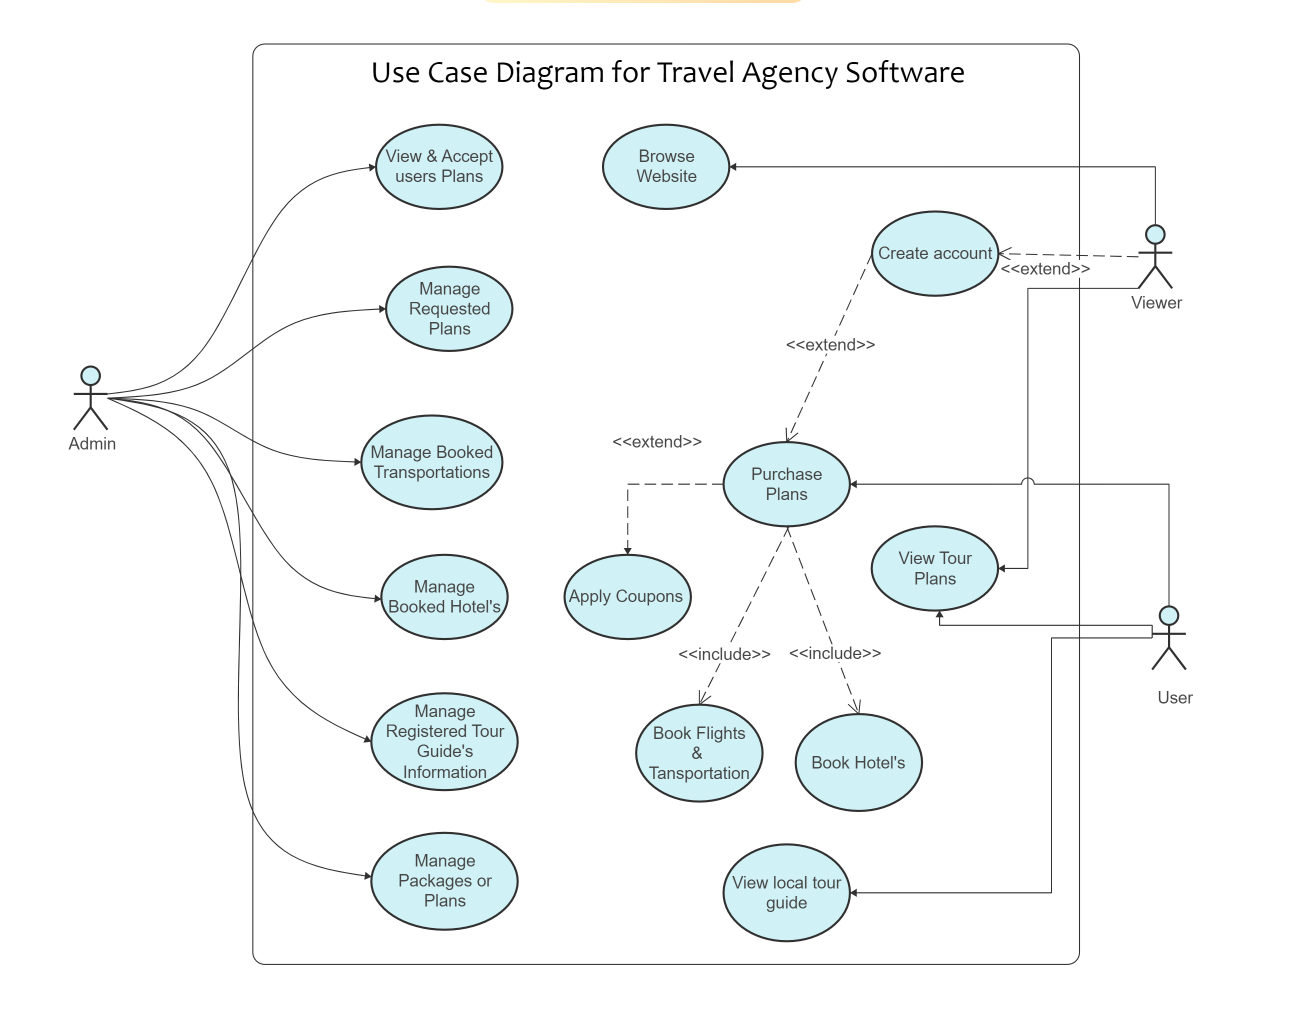
\includegraphics[width=0.8\textwidth]{./figures/Use Case Diagrams/uc_1.3.png} % Replace with your actual Use Case Diagram path
\captionof{figure}{Use Case Diagram for Odyssey Travel Agency Software}
\end{center}
\vspace{0.5cm}

\vspace{0.5cm}
\begin{center}
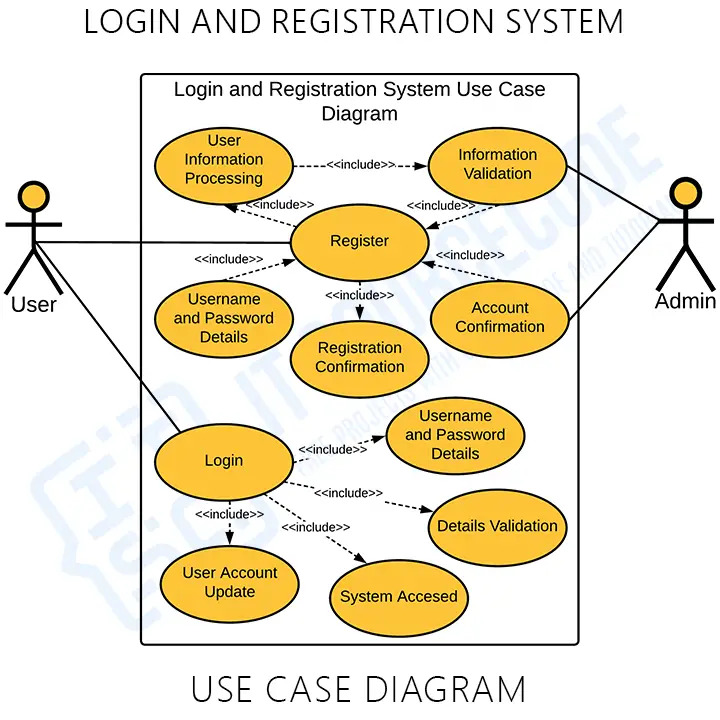
\includegraphics[width=0.8\textwidth]{./figures/Use Case Diagrams/1_usecase.jpg} % Replace with your actual Activity Diagram path
\captionof{figure}{Use Case Diagram Of Login and Registra   tion System} 
\end{center}
\vspace{0.5cm}

\vspace{0.5cm}
\begin{center}
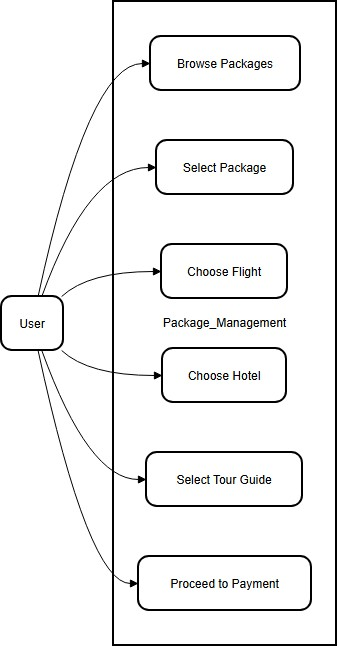
\includegraphics[width=0.5\textwidth]{./figures/Use Case Diagrams/2_usecaase.jpg} % Replace with your actual Activity Diagram path
\captionof{figure}{Package Selection Use Case Diagram}
\end{center}
\vspace{0.5cm}

\vspace{0.5cm}
\begin{center}
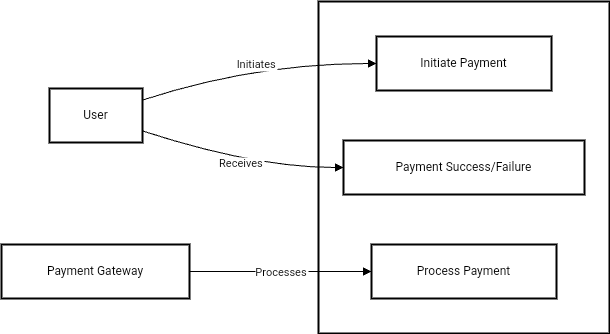
\includegraphics[width=0.8\textwidth]{./figures/Use Case Diagrams/3_usecase.png} % Replace with your actual Activity Diagram path
\captionof{figure}{Payment System Use Case Diagram}
\end{center}
\vspace{0.5cm}

\vspace{0.5cm}
\begin{center}
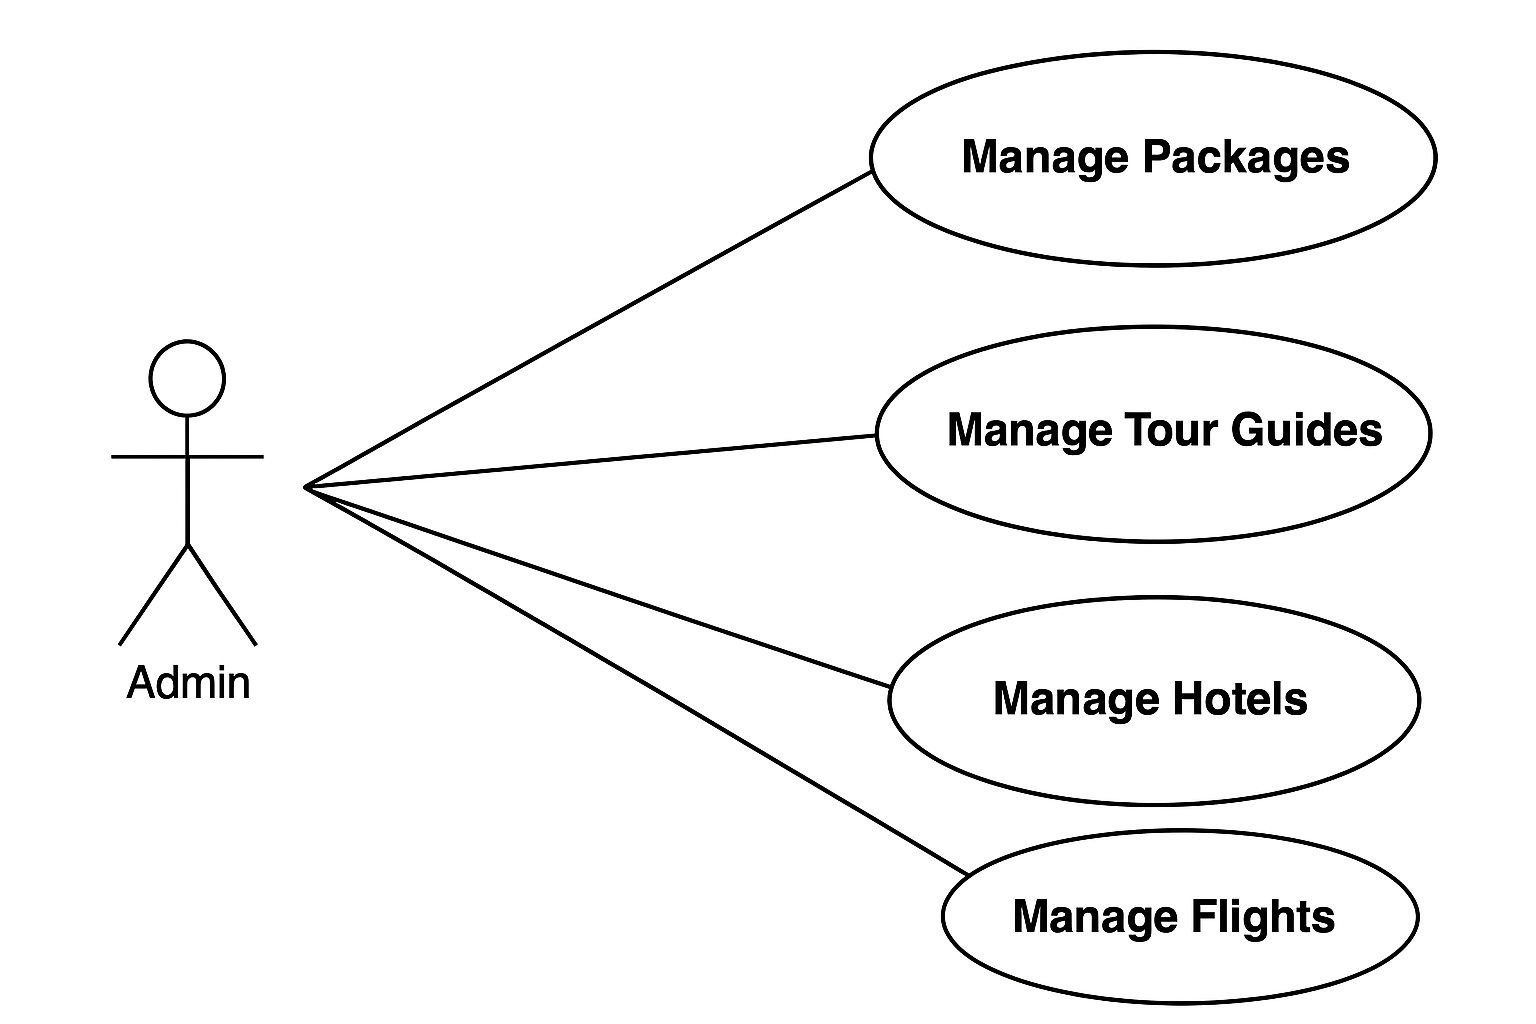
\includegraphics[width=0.8\textwidth]{./figures/Use Case Diagrams/4_crud_usecase.png} % Replace with your actual Activity Diagram path
\captionof{figure}{Admin CRUD Operation Use Case Diagram}
\end{center}
\vspace{0.5cm}

%\newpage
\section{Implementation Details}
This is how you can add a code in the latex template
\begin{lstlisting}[caption={Simple PHP Greeting Function}]
<?php
// PHP example
function greet($name) {
    echo "Hello, " . $name . "!";
}

greet("Alice");
?>
\end{lstlisting}

\newcolumntype{L}[1]{>{\raggedright\arraybackslash}p{#1}}


\section{Testing}
To ensure the reliability and correctness of the Odyssey Travel Agency Software, a structured testing methodology was followed throughout the development lifecycle. This methodology included four primary types of testing:

\begin{itemize}
    \item \textbf{Unit Testing:} Conducted on individual functions and components such as the login system, package listing, and hotel selection module. JavaScript-based unit tests were created using testing libraries like Jest.
    
    \item \textbf{Integration Testing:} Focused on verifying the interaction between modules. For example, integration of the package selection page with the booking module and the payment gateway was carefully validated.
    
    \item \textbf{System Testing:} The complete software was tested in a controlled environment to ensure it meets functional and non-functional requirements. This was done using the deployed system with sample user flows.
    
    \item \textbf{User Acceptance Testing (UAT):} Selected users were invited to test the application from a real-world user perspective. Feedback was collected and evaluated to improve usability, performance, and correctness.
\end{itemize}

\section{Unit Testing}
Unit testing was conducted to test individual modules in isolation. The main goals were to verify correctness of logic, detect early bugs, and ensure maintainability.

\begin{itemize}
    \item Each React component and backend API endpoint was tested using automated test cases.
    \item Modules like authentication, registration, tour guide assignment, and package search were tested individually.
    \item Edge cases were tested such as invalid email formats, empty form submissions, and duplicate user entries.
\end{itemize}

Sample assertion example for user registration:
\begin{verbatim}
expect(registerUser("test@mail.com", "password123")).toBeTruthy();
\end{verbatim}

\section{Integration Testing}
Integration testing was carried out to ensure seamless communication between various components.

\begin{itemize}
    \item Verified data flow from front-end forms to the backend database via the Express API.
    \item Ensured synchronization between hotel/flight selection and the final booking confirmation.
    \item Checked for error handling during API failures or slow network conditions.
\end{itemize}

For example, a package booked by the user was tested to ensure the details were stored correctly and retrievable under the user's booking history.

\section{System Testing}
System testing evaluated the behavior of the complete application. Both functional and non-functional requirements were validated.

\begin{itemize}
    \item Complete booking workflows were tested – from login to payment confirmation.
    \item Admin panel functionalities such as package CRUD operations and tour guide assignment were fully validated.
    \item Tested across multiple browsers (Chrome, Firefox, Edge) to ensure UI consistency.
\end{itemize}

All modules worked correctly when deployed via a local server using XAMPP and MySQL database integration.

\section{User Acceptance Testing}
UAT was performed with a group of 5 users including students and travelers. Their task was to use the system and provide usability feedback.

\begin{itemize}
    \item Majority found the interface intuitive and easy to navigate.
    \item Suggestions were made to improve hotel filtering and add date-based filtering in future versions.
    \item No major bugs were reported during this phase, indicating system readiness.
\end{itemize}

User feedback was recorded and considered for future iteration plans.

\section{Test Cases and Results}
A set of planned test cases were executed to validate the system’s critical functions. A sample of these test cases is summarized below:


\begin{longtable}{|L{6cm}|L{10cm}|}
    \caption{Project Information Table} \label{tab:project_info} \\
    \hline
    \textbf{Project Name} & Odyssey Travel Agency Software
    \\ \hline
    \textbf{Module Name} & Software Testing \\ \hline
    \textbf{Created By} & Hafizur Rahman Sakib and Arnab Shikder \\ \hline
    \textbf{Date of Creation} & 17.02.2024 \\ \hline
    \textbf{Date of Review} & 02.05.2025 \\ \hline
  \end{longtable}

\begin{longtable}[
    ]{
      |L{1.3cm}|L{2.2cm}|L{2.0cm}|L{2.5cm}|L{2.0cm}|L{2.2cm}|L{1.3cm}|
    }
    \caption{Comprehensive Test Case Execution Table for Odyssey Travel Agency Software} \label{tab:test_cases} \\
    \hline
    \textbf{Test Case ID} & 
    \textbf{Test Scenario} & 
    \textbf{Pre-Condition} & 
    \textbf{Test Steps} & 
    \textbf{Test Data} & 
    \textbf{Expected Result} & 
    \textbf{Status} \\
    \hline
    \endfirsthead
    \caption[]{Comprehensive Test Case Execution Table (Continued)} \\
    \hline
    \textbf{Test Case ID} & 
    \textbf{Test Scenario} & 
    \textbf{Pre-Condition} & 
    \textbf{Test Steps} & 
    \textbf{Test Data} & 
    \textbf{Expected Result} & 
    \textbf{Status} \\
    \hline
    \endhead
    \hline
    \endfoot
    \footnotesize % Use smaller font size for better fit
    TC001 & User Login & User is registered & Enter email and password, click login & Email: user@mail.com, Password: 1234 & Dashboard is shown & Pass \\ \hline
    TC002 & Add New Package & Admin is logged in & Go to ``Add Package'', fill form, click submit & Package Name: Beach Trip & Package added successfully & Pass \\ \hline
    TC003 & Invalid Booking & User logged in & Try booking a package skipping hotel selection & N/A & Error message displayed & Pass \\ \hline
    TC004 & Payment Processing & User is on payment page & Enter valid card details and submit & Card No: 4111 1111 1111 1111 & Payment confirmation message & Pass \\ \hline
    TC005 & Session Timeout & User is logged in & Wait 30 minutes without interaction & Timer: 30 mins & Session timeout message shown & Pass \\ \hline
    TC006 & Search Function & User is on homepage & Type keyword in search bar and click search & Keyword: Cox's Bazar & Related packages shown & Pass \\ \hline
    TC007 & Unauthorized Access & User is logged out & Try accessing \texttt{/admin} directly in browser & URL: /admin & Access denied or redirected to login & Pass \\ \hline
    TC008 & User Registration & N/A & Fill in name, email, password, and submit & Name: John Doe, Email: john@mail.com, Password: 1234 & Registration successful message & Pass \\ \hline
    TC009 & Password Reset & User is on login page & Click ``Forgot Password'', enter email, click submit & Email: john@mail.com & Password reset link sent to email & Pass \\ \hline
    TC010 & Edit Package & Admin is logged in & Go to ``Edit Package'', change details, click save & Package ID: 101, New Price: 5000 & Package details updated successfully & Pass \\ \hline
    TC011 & Verify User Logout & User is logged in & Click logout button & N/A & User is logged out & Pass \\ \hline
    TC012 & Invalid Payment & User is on payment page & Enter invalid card details and submit & Card No: 1234 5678 9012 3456 & Error message displayed & Pass \\ \hline
    TC013 & Change User Role & Admin is logged in & Go to user list, select user, change role, click save & User ID: 102, New Role: Admin & User role updated successfully & Pass \\ \hline
    TC014 & User Profile Update & User is logged in & Go to profile page, update name, click save & Name: John Doe $\to$ Jane Doe & Profile updated successfully & Pass \\ \hline
    TC015 & Package Filter & User is on homepage & Apply filters by location and price & Location: Cox's Bazar, Price Range: 3000--5000 & Filtered packages are shown & Pass \\ \hline
    TC016 & Cancel Booking & User is logged in, has a confirmed booking & Go to bookings, select booking, click cancel & N/A & Booking canceled successfully & Pass \\ \hline
    TC017 & Admin Login Attempt & Admin is registered & Enter invalid email or password & Email: admin@mail.com, Password: wrongpassword & Error message displayed & Pass \\ \hline
    TC018 & Package Booking Limit & User is logged in & Try booking a package with exceeded limit & Package Name: Deluxe Tour, Max Bookings: 10 & Error message displayed & Pass \\ \hline
  \end{longtable}
\section{Bug Tracking and Resolution}
Throughout development, bugs were tracked using GitHub Issues. Each bug was logged with the following attributes: ID, title, severity (High/Medium/Low), module affected, and resolution status.

\begin{itemize}
    \item Critical bugs like broken redirects and duplicate booking entries were prioritized.
    \item Weekly triage meetings were held to resolve open bugs collaboratively.
    \item Bugs were documented and tested again after fixes were applied.
\end{itemize}

An example bug entry:
\begin{itemize}
    \item \textbf{ID:} \#24
    \item \textbf{Title:} Booking confirmation not loading
    \item \textbf{Severity:} High
    \item \textbf{Status:} Fixed in Sprint 3
\end{itemize}

\section{Performance and Load Testing}
Performance testing focused on response time, page load time, and system behavior under simulated concurrent users.

\begin{itemize}
    \item Simulated 20 concurrent users performing bookings simultaneously.
    \item Response time remained under 2 seconds for 95\% of operations.
    \item Load testing confirmed the Node.js backend and MySQL database handled concurrent transactions reliably.
\end{itemize}

Future improvements may include caching and CDN integration to boost performance further.

\section{Security Testing}
To ensure data integrity and user protection, security testing was conducted.

\begin{itemize}
    \item Passwords stored in encrypted format using bcrypt.
    \item User inputs validated server-side to prevent SQL Injection and XSS attacks.
    \item JWT-based authentication ensured secure access to protected endpoints.
    \item HTTPS enforced during deployment simulation to protect data in transit.
\end{itemize}

These steps ensured compliance with basic web security standards.

The testing phase validated that the Odyssey Travel Agency Software met all functional and non-functional requirements. It performed reliably across different scenarios, resisted invalid input, and provided a secure and user-friendly interface. The successful completion of unit, integration, system, and acceptance testing confirmed the system's readiness for deployment and future scaling.


\section{Challenges and Solutions}
\section{Conclusion}

The primary goal of this project was to develop a system capable of detecting diseases in cassava leaves while ensuring a smooth and pleasant user experience for farmers. We evaluated six state-of-the-art CNN architectures—Xception, EfficientNetB0, ResNet50, VGG16, DenseNet121, and InceptionV3—alongside our proposed ReXNet150 model. 

On the validation set, Xception achieved an accuracy of 91.3 % with an F1–score of 91.0 %, while EfficientNetB0 reached 91.1 % accuracy and 90.8 % F1–score. ResNet50, DenseNet121, and InceptionV3 delivered moderate performance with accuracies of 85.0 %, 87.0 %, and 86.4 %, and F1–scores of 84.6 %, 86.8 %, and 86.0 %, respectively. VGG16 lagged behind with 68.0 % accuracy and a 67.5 % F1–score. Our ReXNet150 model outperformed all others, achieving a validation accuracy of 94.7 % and an F1–score of 94.9 %.

These results demonstrate that ReXNet150 provides the best balance between classification accuracy and computational efficiency for cassava leaf disease detection. While the high performance of Xception and EfficientNetB0 confirms their suitability for this task, ReXNet150’s superior metrics make it the preferred choice for real-world deployment.

\section{Future Work}

To further enhance and expand this system, we plan to:
\begin{itemize}
    \item \textbf{Fine-tune ReXNet150 further,} exploring additional hyperparameter optimizations and architectural refinements.
    \item \textbf{Investigate newer and lightweight architectures,} aiming to improve the speed–accuracy trade-off.
    \item \textbf{Apply model compression techniques} such as pruning, quantization, and knowledge distillation, enabling real-time inference on mobile and edge devices.
    \item \textbf{Develop a mobile application} for on-the-spot disease diagnosis, empowering farmers without requiring internet connectivity.
    \item \textbf{Expand the dataset} by collecting images from diverse geographical regions and environmental conditions to bolster model generalization.
    \item \textbf{Extend the framework to other crops,} creating a universal plant disease detection platform.
\end{itemize}

This work lays a solid foundation for intelligent, accessible solutions in agricultural disease management. Future researchers and practitioners can build upon our findings to develop even more robust and versatile systems.

%\newpage
\appendix
\section{Project Timeline}
\begin{figure}
    \centering
    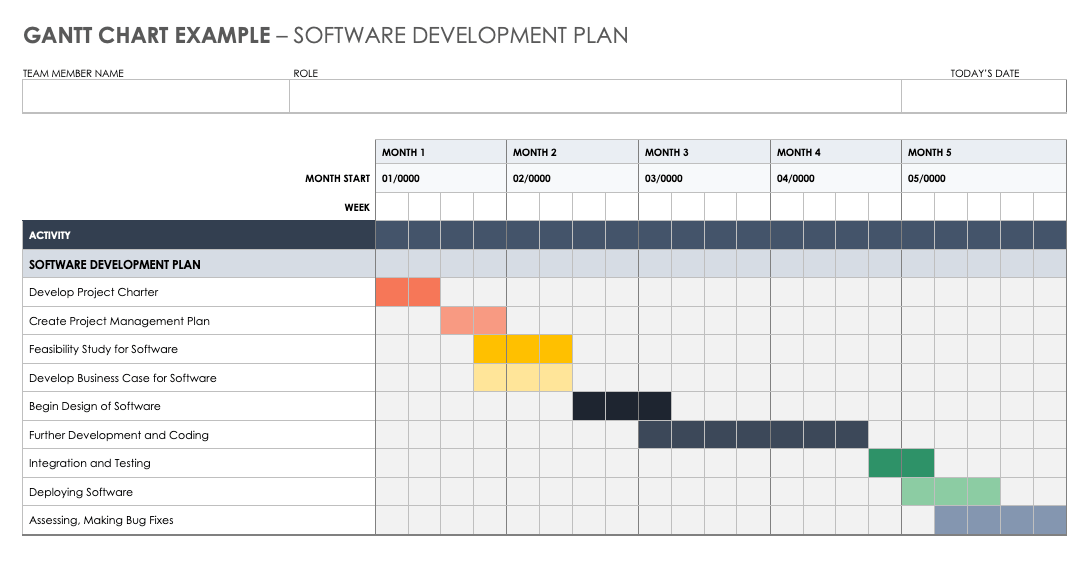
\includegraphics[width=1.2\linewidth, angle=90]{IC-Gantt-Chart-.png}
    \caption{Enter Caption}
    \label{fig:enter-label}
\end{figure}


% References
\newpage
\phantomsection
\addcontentsline{toc}{section}{REFERENCES}
\bibliographystyle{IEEEtran}
\bibliography{biblio} % Ensure biblio.bib exists
\end{document}